% Kapania2014_DSCC_Draft.tex
%================================================
% $Id: ifacconf.tex 17 2008-12-16 15:13:36Z jpuente $
% Template for IFAC meeting papers
% Copyright (c) 2007-2008 International Federation of Automatic Control
%================================================
\documentclass[twocolumn,10pt]{asme2e}

%% Replace here with information related to your conference
\confshortname{DSCC 2014} \conffullname{ASME 2014 Dynamic
Systems and Control Conference} \confdate{22-24}
\confmonth{October} \confyear{2014} \confcity{San Antonio,
Texas} \confcountry{USA}

%% Replace DETC2005-12345 with the number supplied to you
%% by ASME for your paper.
\papernum{DSCC2012-8585}

%===============================================================================
\usepackage{graphicx}   % include this line if your document contains figures
\usepackage{psfrag}
\usepackage{color}
\usepackage{epstopdf}
\usepackage{amssymb,amsmath}
\usepackage{multirow}
\usepackage{ctable}
\usepackage{amsfonts}
  \newcommand{\field}[1]{\mathbb{#1}}


\title{State-Dependent Feedforward Steering for Vehicle Handling at the Limits of Tire Adhesion}

%%% first author
\author{Nitin R. Kapania\thanks{Corresponding author.}
    \affiliation{
    Dynamic Design Lab\\
    Dept. of Mechanical Engineering\\
    Stanford University\\
    Stanford, California 94305\\
    email: nkapania@stanford.edu
    }	
}

\author{J. Christian Gerdes
    \affiliation{
    Dynamic Design Lab\\
    Dept. of Mechanical Engineering\\
    Stanford University\\
    Stanford, California 94305\\
    email: gerdes@stanford.edu
    }
}

\begin{document}

\maketitle

%%%%%%%%%%%%%%%%%%%%%%%%%%%%%%%%%%%%%%%%%%%%%%%%%%%%%%%%%%%%%%%%%%%%%%
\begin{abstract} 
\it{This paper presents a simple feedforward-feedback control architecture for autonomous steering control at the limits of tire-road friction, 
and discusses an approach for computation of the feedforward (FFW) steering command. The feedforward control utilizes vehicle state information, namely vehicle yaw rate and sideslip, to provide a feedforward steering input seeking to eliminate path tracking dynamics of a fixed point on the vehicle. The vehicle center of percussion (COP) is used as a convenient point to 
base the feedforward steering, and an observer is developed to estimate the required vehicle states from a nonlinear two-state bicycle model. Experimental performance is presented on an Audi TTS testbed cornering at lateral accelerations of up to .9 g on a closed-course race circuit. Finally, sensitivity of the feedforward method to modelling error is analyzed through simulation.}
\end{abstract}

%%%%%%%%%%%%%%%%%%%%%%%%%%%%%%%%%%%%%%%%%%%%%%%%%%%%%%%%%%%%%%%%%%%%%%
%\begin{nomenclature}
%\entry{CA50}{Crank angle whereby 50\% of the fuel has been consumed.}
%\entry{IMEP}{Indicated mean effective pressure}
%\end{nomenclature}

%%%%%%%%%%%%%%%%%%%%%%%%%%%%%%%%%%%%%%%%%%%%%%%%%%%%%%%%%%%%%%%%%%%%%%
\section{INTRODUCTION}

There have been many active steering controllers proposed and implemented for autonomous vehicles in recent years. For these systems, careful design of the feedforward steering is important is vital for minimizing the needed feedback control effort and enabling smooth lateral tracking performance. As part of preliminary research in the early 1990's with the California PATH program, Shladover et al. \cite{shladover} proposed
a feedforward control law based on a linear vehicle model and accounting for longitudinal dynamics.  In the early 2000's,  Mammar and Koenig  developed a combined feedforward/feedback system for shared vehicle control with a human driver, with the feedforward steering acting to minimize yaw rate tracking error over a wide range of possible plant perturbations \cite{mammar}. Curvature-based feedforward control in combination with feedback on lateral offset and heading error
was used in the Honda Advanced Safety Vehicle (ASV) \cite{takahashi}. A similar approach was used in 2005 for California Institute of Technology's vehicle in the DARPA Urban Challenge \cite{cremean}. 

Feedforward control based on linear vehicle models is suitable for everyday driving conditions, but to ensure passenger safety in emergency safety maneuvers, such as low-friction or obstacle avoidance situations, autonomous steering systems must achieve both stability and accurate tracking of a reference path at the physical limits of tire adhesion. Previous work at the limits of handling
includes development by Kritayakirana and Gerdes of a combined steering and longitudinal controller inspired by race car drivers \cite{mickgeneral}. The authors later demonstrated better
handling at the friction limits using a non-linear reference model accounting for tire saturation at high lateral acceleration \cite{mickcop}. 

This paper further extends research on feedforward steering control at the limits of handling, building on the idea 
presented in \cite{mickcop} of using feedforward control to eliminate path tracking dynamics at a fixed point on the vehicle. Practical concerns for implementation at high lateral acceleration is addressed, particularly the need for an observer to provide estimates of vehicle lateral velocity and yaw rate
for accurate computation of the feedforward road wheel angle $\delta$. Experimental performance over four turns on a 1.3 km stretch of racetrack is shown to be desirable at lateral accelerations of up to .85 g, with susceptibility 
to underdamped vehicle oscillation occurring at higher lateral acceleration ($ a_y> .9$ g). A numerical simulation is developed to explain potential causes for this behavior.


%%%%%%%%%%%%%%%%%%%%%%%%%%%%%%%%%%%%%%%%%%%%%%%%%%%%%%%%%%%%%%%%%%%%%%
\section{CONTROLLER OVERVIEW} \label{sec:modeling}

A block digram of the overall controller structure is shown in Figure \ref{fig:blockDiagram}. The desired path curvature 
for the vehicle to follow is provided to the controller via a separate path planning algorithm 
(see \cite{theodosis}). Additionally, the longitudinal velocity profile is obtained from a longitudinal 
controller that keeps the combined lateral/longitudinal acceleration magnitude of the vehicle at a specified value (see \cite{mickgeneral}). The 
feedforward steering input, to be explored in this paper, provides a FFW roadwheel angle $\delta_{FFW}$ for the vehicle to track. Path tracking error states $e$ and $\Delta\Psi$ are used
for a lanekeeping feedback algorithm. 

%%%%%%%%%%%%%%%%% FIGURE         blockDiagram
\begin{figure}
\centering
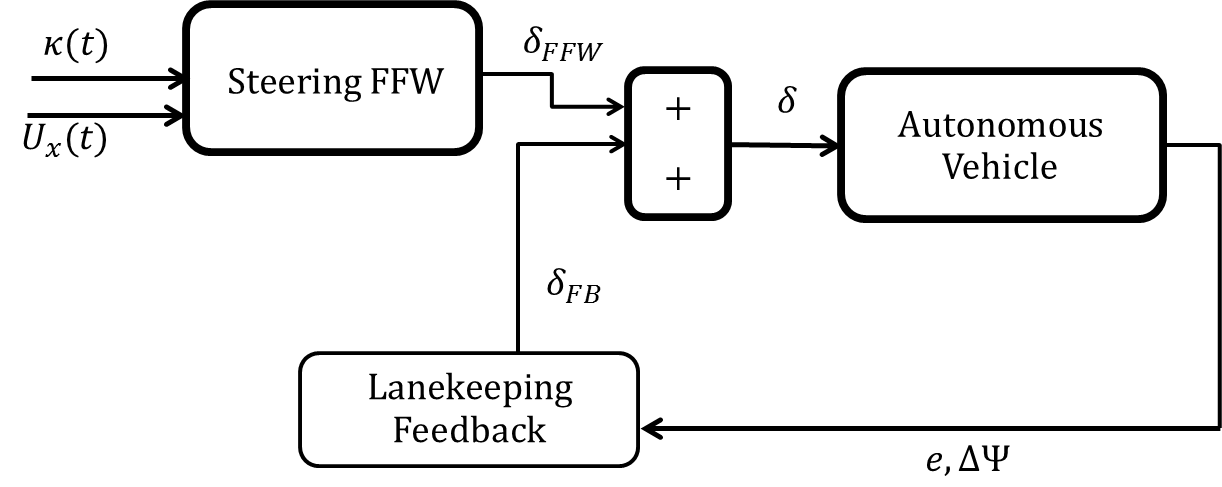
\includegraphics[width=3.25in]{figure/blockDiagram.png}
\caption{Block diagram of feedforward-feedback steering controller.}
\label{fig:blockDiagram}
\end{figure}

\subsection{Lanekeeping Feedback}
Figure \ref{fig:lookahead} shows a vehicle cornering at an offset to a desired path. The lateral distance from the vehicle's center of gravity to the path tangent is defined as the lateral offset error, $e$, and the angle between the vehicle's heading and the
desired path heading is denoted by $\Delta\Psi$. The dynamics of the error states are given by

\begin{equation}
\begin{aligned}
\dot{e} = U_y\cos(\Delta\Psi)+U_x\sin(\Delta\Psi)\\
\dot{\Delta\Psi} = \dot{r} - \kappa\dot{s}
\end{aligned}
\label{eqn:errordynamics}
\end{equation}

Where $\kappa$ is the road curvature and $s$ is distance along the path. The lanekeeping module creates a feedback steer angle based proportionally on lookahead distance, $e_{LA}$:

\begin{equation}
\begin{aligned}
\delta_{FB} = -k_p(e_{LA} )\\
e_{LA} = e+x_{LA}\sin(\Delta\Psi)
\label{eqn:fbeqn}
\end{aligned}
\end{equation}

Where the ``lookahead distance" $e_{LA}$ is a weighted sum of path offset error $e$ and heading error $\Delta\Psi$.
Feedback based on tracking a lookahead error $e_{LA}$ has been studied extensively in the literature. Heuristics for selection of lookahead distance $x_{LA}$ and proportional gain $k_p$ 
are shown in \cite{rosseter}, and  desirable stability
properties over significant front and rear tire saturation levels is demonstrated in \cite{talvala}. Stability at the physical limits of handling is also shown experimentally in \cite{mickthesis}.


\begin{figure}
\centering
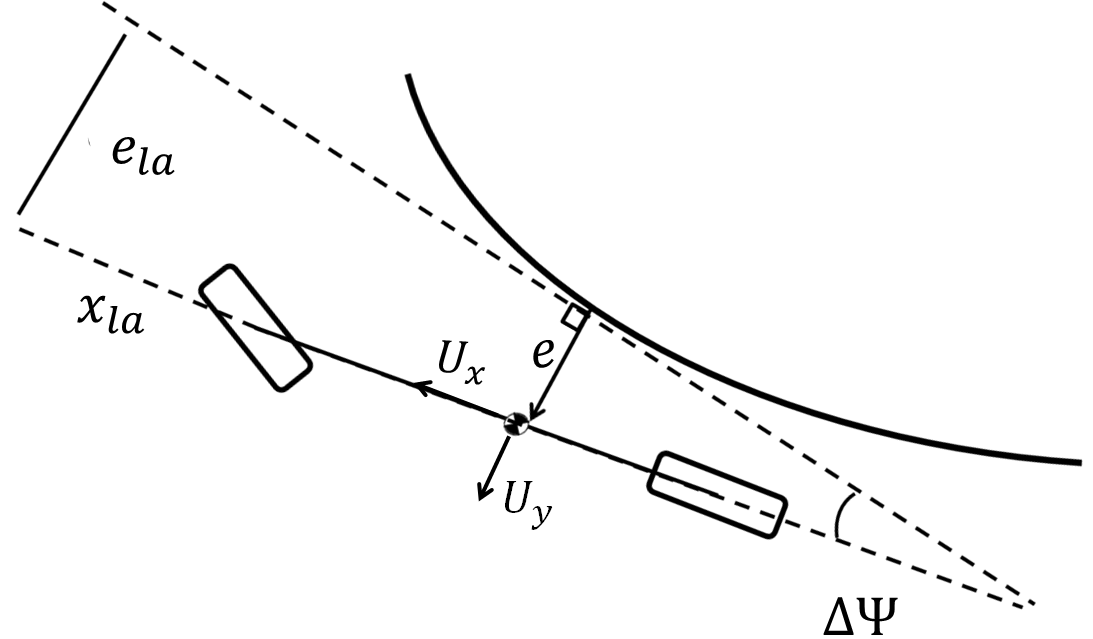
\includegraphics[width=2.5in]{figure/lookahead.png}
\caption{Schematic showing error states $e$ and $\Delta\Psi$ for a simplified fixed-track vehicle.}
\label{fig:lookahead}
\end{figure}


\subsection{Experimental Setup}

\begin{figure}
\centering
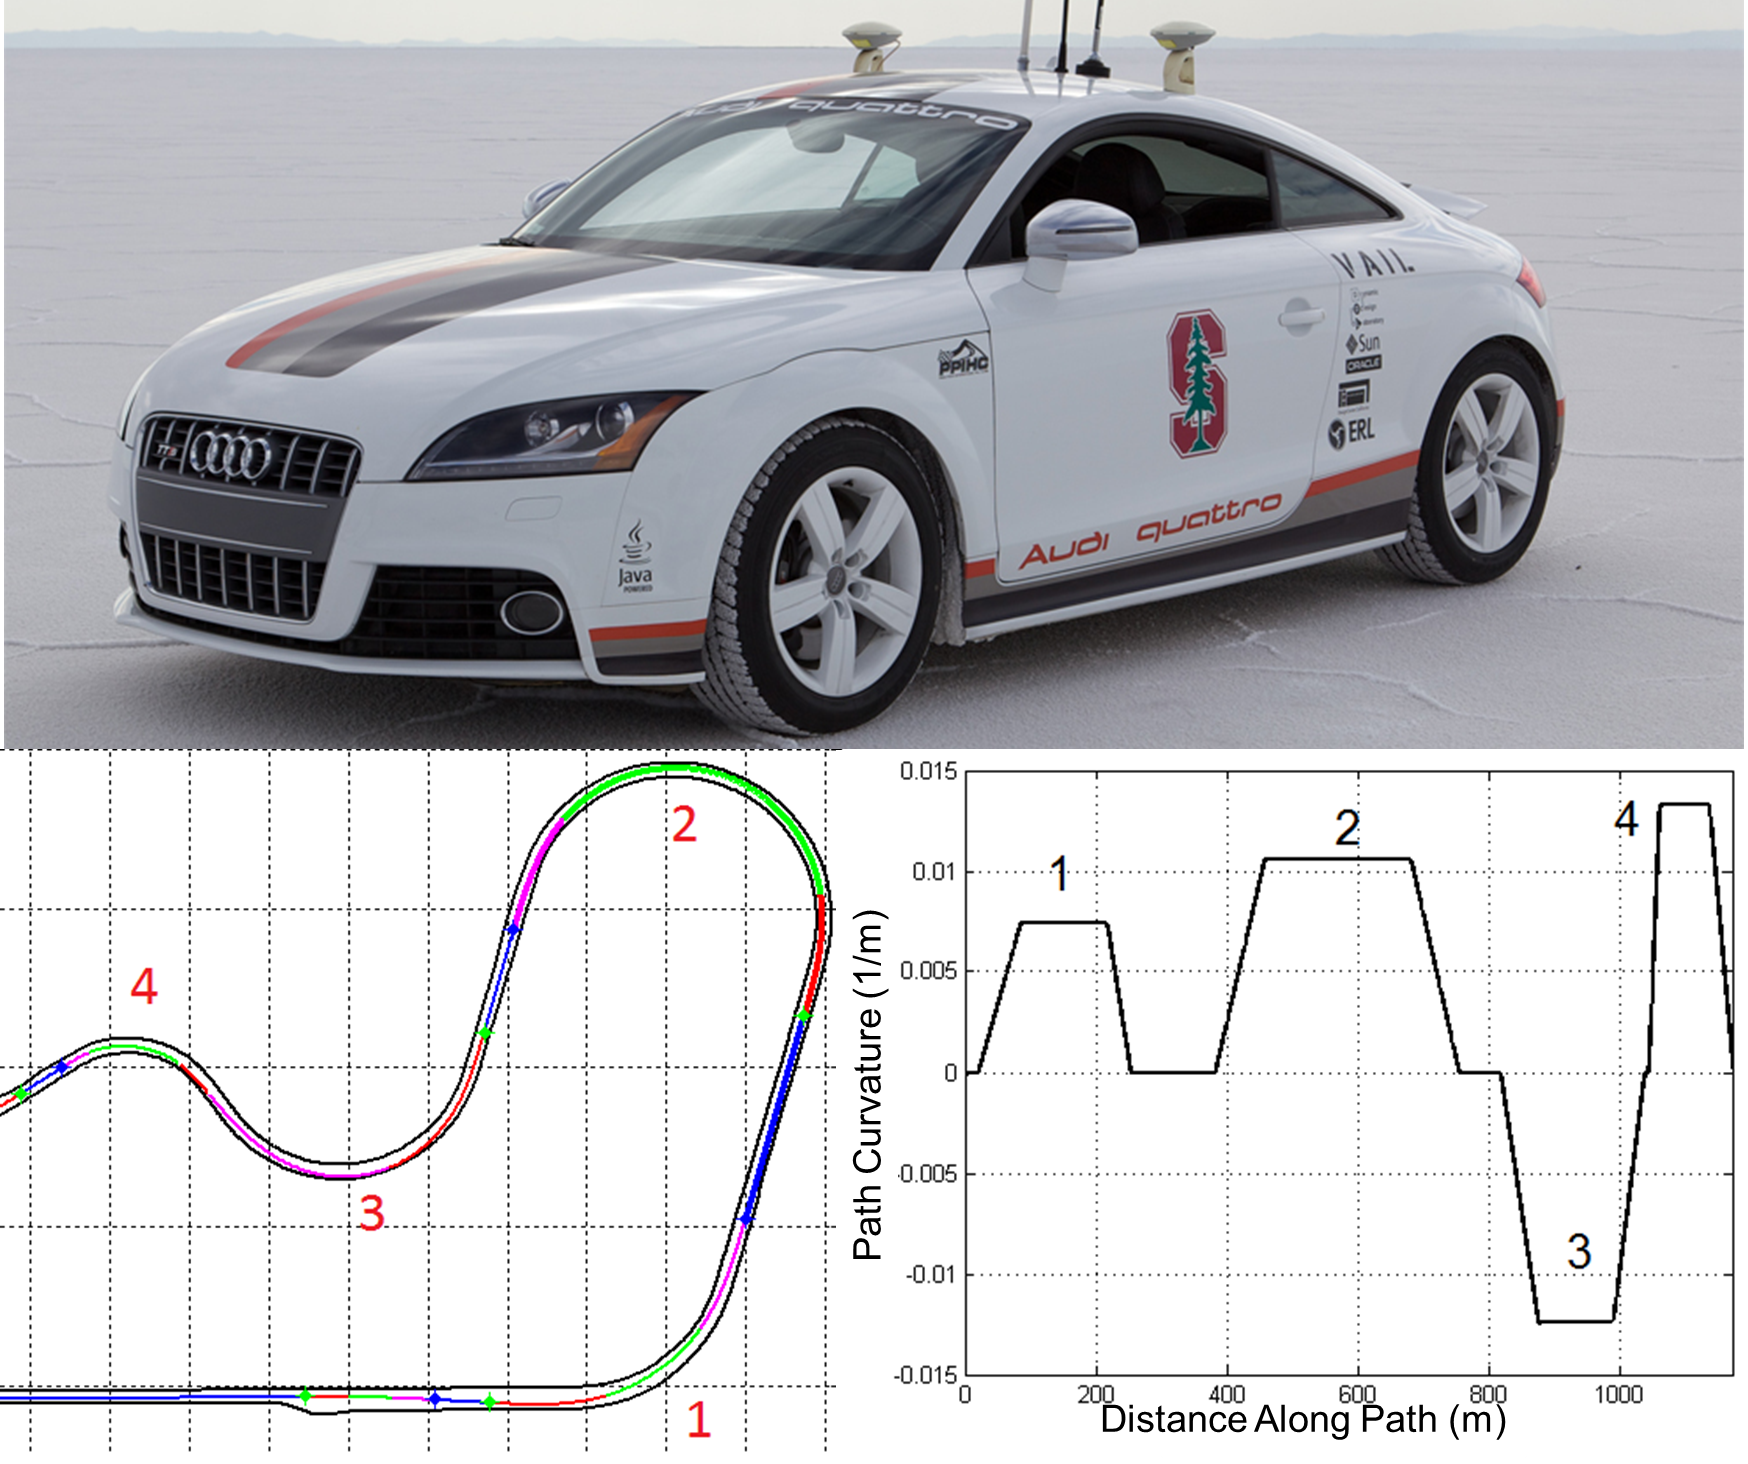
\includegraphics[width=3.25in]{figure/experimentInfo.png}
\caption{(Top) Audi TTS vehicle used for experimental testing (Bottom Left) Overhead view of first four turns of Thunder Hill Raceway Park along with desired trajectory. Blue lines denote straight paths, green denotes constant curvature sections, and red/magenta denote transitional segments with linearly varying curvature.
(Bottom Right) Curvature of track as function of distance. }
\label{fig:shelleyPic}
\end{figure}

All vehicle data is collected on a four-wheel drive Audi TTS (Figure \ref{fig:shelleyPic}) equipped with an electronic power steering motor,
active brake booster, and throttle by wire. Data was collected over a 1.3 km stretch of paved road (friction coefficient $\mu \approx 1$) at Thunder Hill Raceway Park in Willows, CA, with curvature profile shown
in \ref{fig:shelleyPic}. An integrated differential Global Positioning System (DGPS) and Inertial Navigation System (INS) is utilized to obtain global vehicle positions and states.  A map matching algorithm
algorithm (\cite{rosseter}) synthesizes information from the DGPS/INS system to obtain the $e$ and $\Delta\Psi$ in Figure \ref{fig:lookahead}. The controller operates at a 200 Hz sampling rate.




\section{FEEDFORWARD TRACKING OF CENTER OF \\ PERCUSSION} \label{cop}

The motivation for the first feedforward algorithm is inspired by \cite{mickcop} and comes from the two-state planar bicycle model for a vehicle, shown with relevant states and geometric properties in Figure \ref{fig:bikemodel}. Vehicle states of yaw rate $r$ and lateral velocity $U_y$ have the following equations of motion:

\begin{equation}
\begin{aligned}
F_{yf} + F_{yr} = m(\dot{U_y} + U_xr)\\
aF_{yf} - bF_{yr} = I_zz\dot{r}
\label{eqn:eom}
\end{aligned}
\end{equation}

\begin{figure}
\centering
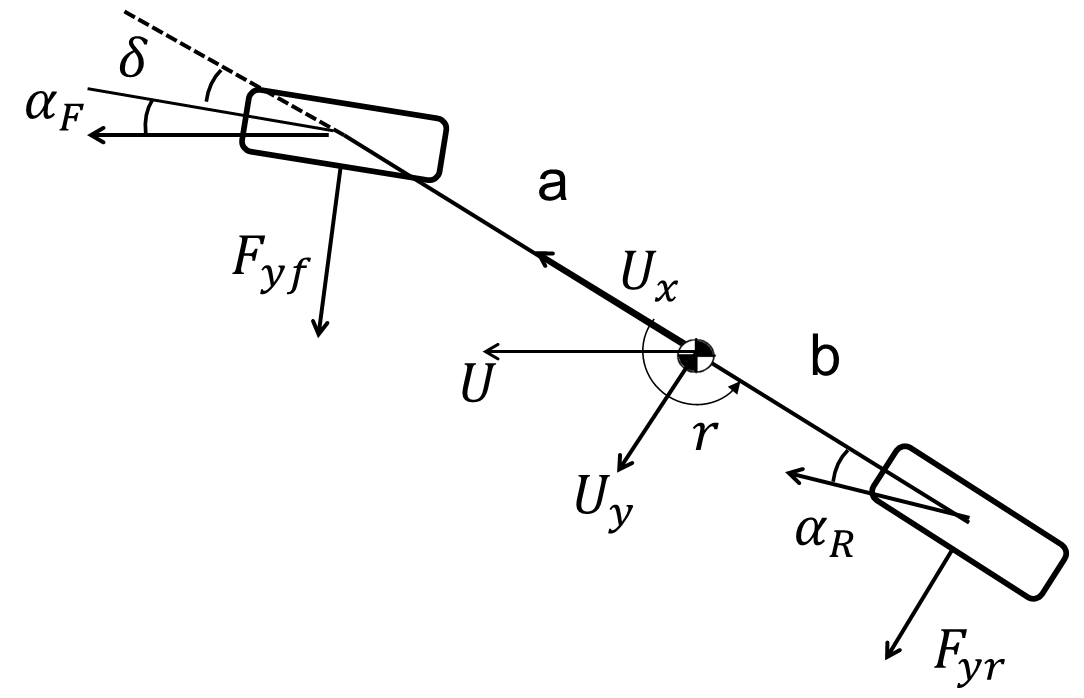
\includegraphics[width=2.5in]{figure/bikemodel.png}
\caption{Schematic of planar, two-wheel bicycle model. Vehicle states are yaw rate $r$ and lateral velocity $U_y$. Vehicle speed $U_x$ is held constant. Front and rear tire slips are denoted by $\alpha_{F}$ and $\alpha_{R}$}
\label{fig:bikemodel}
\end{figure}


Where the planar yaw moment of inertia is given by $I_z$ and the longitudinal speed $U_x$ is assumed constant. The underlying
goal of this feedforward algorithm is to keep a vehicle-fixed point $x_p$ located on the desired trajectory at all time. The lateral error $e_p$ at point $x_p$ is given by 

\begin{equation}
e_p = e + x_p\sin(\Delta\Psi)
\label{eqn:epeq}
\end{equation}

Kritayakirana and Gerdes \cite{mickcop} note that a convenient choice for $x_p$ is the vehicle center of percussion, $x_{cop} = \frac{I_{zz}}{bm}$.
Taking second derivatives of (\ref{eqn:epeq}) with $x_p = x_{cop}$ and substituting terms from (\ref{eqn:errordynamics}) and (\ref{eqn:eom}) yields:

\begin{equation}
	\ddot{e_{cop}} = \frac{L}{b}\frac{F_{yf}}{m} - U_x\kappa\dot{s} - x_{cop}(\kappa\ddot{s} + \dot{\kappa}\dot{s})
\label{eqn:ddecop}
\end{equation}

The convenience of choosing a feedforward algorithm to eliminate tracking error at the center of percussion is apparent in (\ref{eqn:ddecop}). The error dynamics at the center of percussion depends only on the 
front force input $F_{yf}$. Setting $e_{cop}$ to 0 yields a feedforward control law for the front tire force:

\begin{equation}
	F^{FFW}_{yf} = \frac{mb}{L}(U_x\kappa\dot{s} + x_{cop}(\kappa\ddot{s} + \dot{\kappa}\dot{s})
\label{eqn:ddecop}
\end{equation}

However, since vehicle steering is ultimately controlled by a steering input $\delta$, an appropriate method for translating $F^{FFW}_{yf}$ into a suitable feedforward steering command $\delta_{FFW}$ is needed. The proposed methodology is illustrated in Figure \ref{fig:observerBD}.

\begin{figure}
\centering
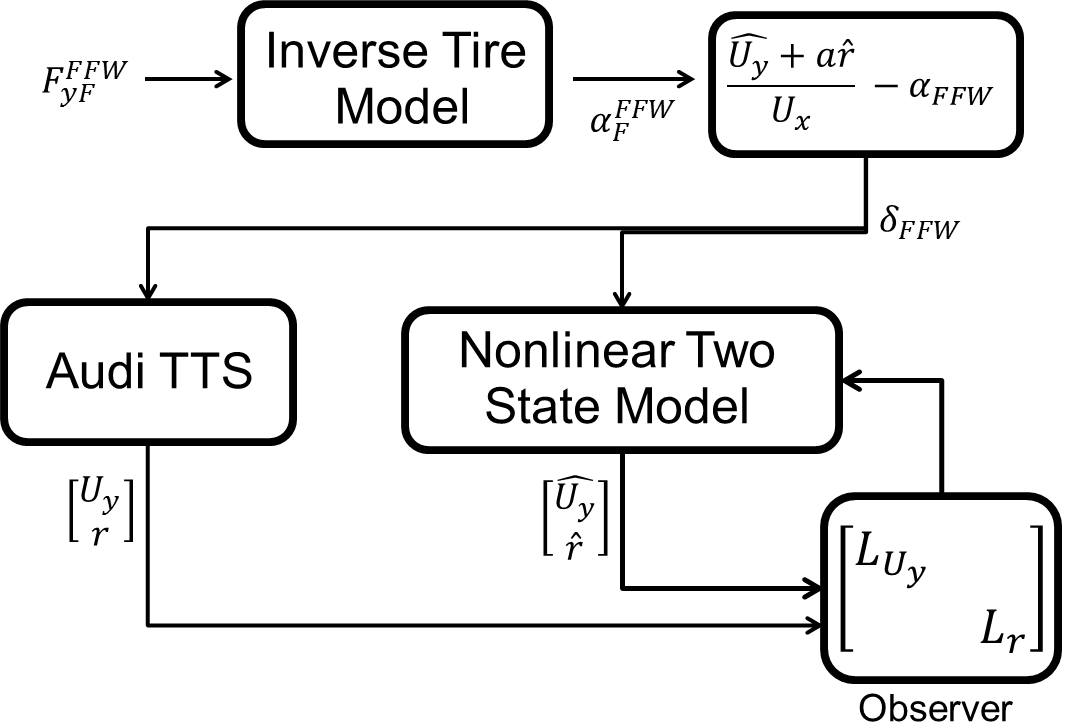
\includegraphics[width=3.25in]{figure/observerBD.png}
\caption{Proposed method for determining $\delta_{FFW}$, using a nonlinear inverse tire model and linear observer.}
\label{fig:observerBD}
\end{figure}

The front feedforward tire force is converted into a feedforward front tire slip $\alpha^{FFW}_F$ through an inverted tire model. Successful handling at the friction limits requires a tire model accounting for saturation of tire force
with increasing tire slip magnitude, so a single friction coefficient Fiala model \cite{pacejka2012} is used: 

\begin{eqnarray}
	F_\mathrm{y}&=&\begin{cases} -C_{\alpha}\tan\alpha + \frac{C_{\alpha}^2}{3\mu F_\mathrm{z}} |\tan\alpha| \tan\alpha \vspace{2mm} \\ \hspace{8mm}- \frac{C_{\alpha}^3}{27\mu^2F_\mathrm{z}^2}\tan^3\alpha,
\hspace{4mm}  |\alpha| < \arctan{\left(\frac{3\mu F_\mathrm{z}}{C_\alpha}\right)} \\ -\mu F_\mathrm{z}\text{sgn} \ \alpha, \hspace{24mm} \mathrm{otherwise} \end{cases} \nonumber\\
&=&f_{\mathrm{tire}}\left(\alpha\right) \label{eqn:fiala}
\end{eqnarray}

where $\mu$ is the surface coefficient of friction, $F_\mathrm{z[f,r]}$ is the normal load, and $C_\alpha$ is the tire cornering stiffness. The desired force $F^{FFW}_{yf}$ is converted to $\alpha^{FFW}_F$
through a lookup table.

\subsection{Yaw Rate - Sideslip Observer}

As Figure \ref{fig:observerBD} indicates, $\alpha^{FFW}_F$ is converted to a steering command through the following vehicle kinematics:

\begin{equation}
	\delta_{FFW} = \frac{\hat{U}_y+a\hat{r}}{U_x}-\alpha^{FFW}_F
\label{eqn:alphaToDelta}
\end{equation}

Sensor values of $U_y$ and yaw rate $r$ are available through the testbed's GPS/INS system. However, at the limits of handling ($a_y > $ .7 g), the underdamped vehicle response coupled with actuation delays creates
an oscillatory feedforward command, as shown experimentally in Figure \ref{fig:noObserver}. To avoid this issue, a two-state bicycle model with state equations given by (\ref{eqn:eom}) and tire model given by (\ref{eqn:fiala}) is set up to run in real time with the vehicle. Simulated values
of $U^{sim}_y$ and $r^{sim}$ are blended with sensor measurements to determine estimated values $\hat{U}_y$ and $\hat{r}$.  Figure \ref{fig:observerBD} shows a diagonal observer structure is chosen with gains $L_{U_y}$  and $L_r$. Values for the
observer gains are tuned experimentally via a logarithmic sweep of feasible gain choices over the section of race track shown in Figure \ref{fig:shelleyPic}.

\begin{figure}
\centering
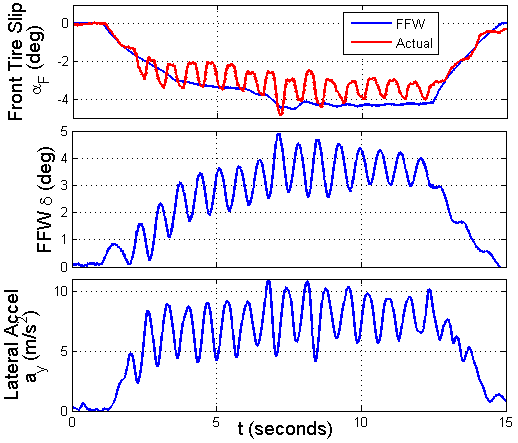
\includegraphics[width=3.25in]{figure/noObserver.png}
\caption{Steering feedforward implementation on Turn 2 (see Figure \ref{fig:shelleyPic}) with no observer at lateral acceleration .7 g. Note the smooth feedforward front tire slip is mapped into a heavily oscillatory steer angle command.}
\label{fig:noObserver}
\end{figure}

\subsection{Experimental Results}

Experimental results with the observer are shown in Figure \ref{fig:withObserver}. Data was obtained by keeping a constant lateral acceleration of .8 g through all corners of the track shown in Figure \ref{fig:shelleyPic}. 
The observer removes the issue of oscillatory feedforward steering commands at the vehicle limits of handling. The front tire slip $\alpha_F$ remains within .5 degrees of the $\alpha^{FFW}_F$ value
computed through the inverted tire model, as the required steering feedback $\delta_{FB}$ is generally low ($|\delta_{FB}| <$ .5 deg). Tracking of the lookahead objective $e_{la}$ remains within .2 meters, although steady
state errors in lateral error $e$ and heading error $\Delta\Psi$ are observed as a known limitation of the lanekeeping feedback system. The relatively low observer gains, shown in Table \ref{params} weight
the estimated states $\hat{U}_y$ and $\hat{r}$ closer to the simulated values versus the sensor measurements. This enables a smoother feedforward command while avoiding issues with path tracking in the case of unmodeled plant dynamics.

\begin{figure}
\centering
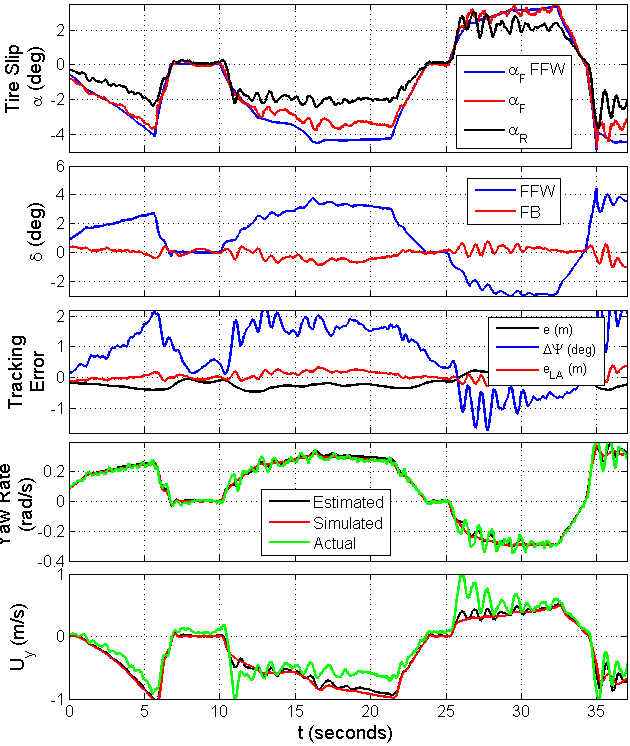
\includegraphics[width=3.25in]{figure/withObserver.png}
\caption{Steering feedforward implementation on Turn 2 (see Figure \ref{fig:shelleyPic}) with no observer at lateral acceleration .7 g. Note the smooth feedforward front tire slip is mapped into a heavily oscillatory steer angle command.}
\label{fig:withObserver}
\end{figure}

\subsection{Sensitivity to Model Mismatch}

With any feedforward algorithm, it is necessary to check controller performance in the event the feedforward model deviates significantly from the actual plant. The feedforward control 
analysed in this paper depends heavily on accurate tracking of transient vehicle states $U_y$ and $r$. This ability of the feedforward to provide accurate steering commands in transient conditions is a benefit for accurate handling at the 
limits, but increases the possibility of an undesirable control input if the  parameters used in the feedforward bicycle model simulation are incorrect, particularly lumped tire parameters $C_f$, $C_r$, and $\mu$ . 

\begin{figure}
\centering
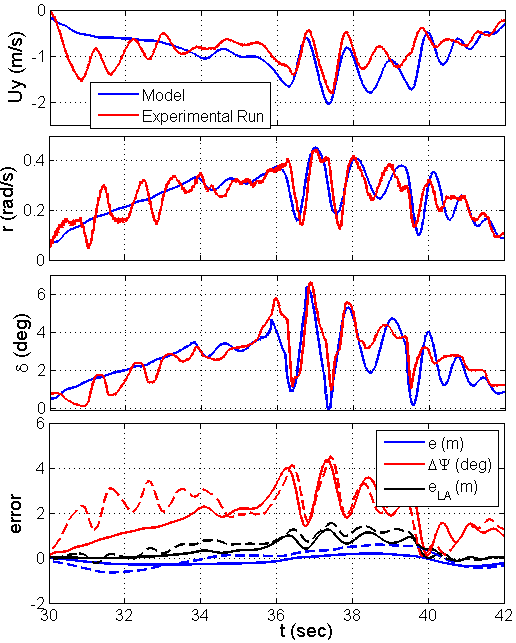
\includegraphics[width=3.25in]{figure/withParameterMismatch.png}
\caption{Steering feedforward implementation on Turn 2 (see Figure \ref{fig:shelleyPic}) with no observer at lateral acceleration .7 g. Note the smooth feedforward front tire slip is mapped into a heavily oscillatory steer angle command.}
\label{fig:withParameterMismatch}
\end{figure}


Figure \ref{fig:withParameterMismatch} shows experimental results when the vehicle operates autonomously at a very high acceleration level (peak $a_y$ = .9 g) on section 2 of the race track. Even with the observer in place, the feedforward steering signal exhibits underdamped oscillations, with the result being an undesirable vehicle yaw rate response that oscillates around \%50 above and
below the steady state yaw rate. An off-line simulation was developed to determine possible causes of the potentially underdamped vehicle response at the very limits of friction.
experiment. The simulation computes the anticipated vehicle response when the friction estimate used by the feedforward control is 10\% too low (i.e $\mu = $ .9 in (\ref{eqn:fiala}). The simulation predicts
predicts vehicle states  using the bicycle model in (\ref{eqn:eom}), with longitudinal dynamics neglected. Error dynamics are predicted from (\ref{eqn:errordynamics}). 

The simulation shows that the feedforward controller can be sensitive to parameter mismatches when operating at extreme lateral accelerations. The model results, overlayed in Figure \ref{fig:withParameterMismatch} exhibit the same underdamped vehicle response seen experimentally. The model matches
particularly well from $t =$ 36 to 40 seconds, when the car is cornering at constant speed and the simulated assumption of neglected longitudinal dynamics is valid. The result indicates that improperly estimated parameters such as tire friction can adversely effect the feedforward algorithm and resulting vehicle response, but typically
only at very high lateral acceleration.





%%%%%%%%%%%%%%%%%%%%%%%%%%%%%%%%%%%%%%%%%%%%%%%%%%%%%%%%%%%%%%%%%%%%%%
\begin{acknowledgment}
Nitin Kapania is supported by a Graduate Research Fellowship from the National Science Foundation.
\end{acknowledgment}

%%%%%%%%%%%%%%%%%%%%%%%%%%%%%%%%%%%%%%%%%%%%%%%%%%%%%%%%%%%%%%%%%%%%%%
% The bibliography is stored in an external database file
% in the BibTeX format (file_name.bib).  The bibliography is
% created by the following command and it will appear in this
% position in the document. You may, of course, create your
% own bibliography by using thebibliography environment as in
%
% \begin{thebibliography}{12}
% ...
% \bibitem{itemreference} D. E. Knudsen.
% {\em 1966 World Bnus Almanac.}
% {Permafrost Press, Novosibirsk.}
% ...
% \end{thebibliography}

% Here's where you specify the bibliography style file.
% The full file name for the bibliography style file
% used for an ASME paper is asmems4.bst.
\bibliographystyle{asmems4}

% Here's where you specify the bibliography database file.
% The full file name of the bibliography database for this
% article is asme2e.bib. The name for your database is up
% to you.
\bibliography{Bibliography}

\end{document}
